
\documentclass[12pt]{article}
\usepackage[paper=letterpaper,margin=2cm]{geometry}

\usepackage{amsmath}
\usepackage{amsthm} %needed for the proofs 
\usepackage{amssymb}
\usepackage{titling}
\usepackage{thmtools}
\usepackage{mathptmx} %font
\usepackage{verbatim} % for comments
\usepackage{mdframed}
\usepackage[linesnumbered,ruled,vlined]{algorithm2e}
\usepackage{lipsum}

\usepackage[T1]{fontenc} %header
\usepackage[utf8]{inputenc}%header
\usepackage{geometry} %header
\usepackage{fancyhdr}%header

\usepackage{forest} % for decision trees

%images
\usepackage{graphicx}
\graphicspath{ {./graphics/} }
% to include an image, do: 
%    \begin{center}
%    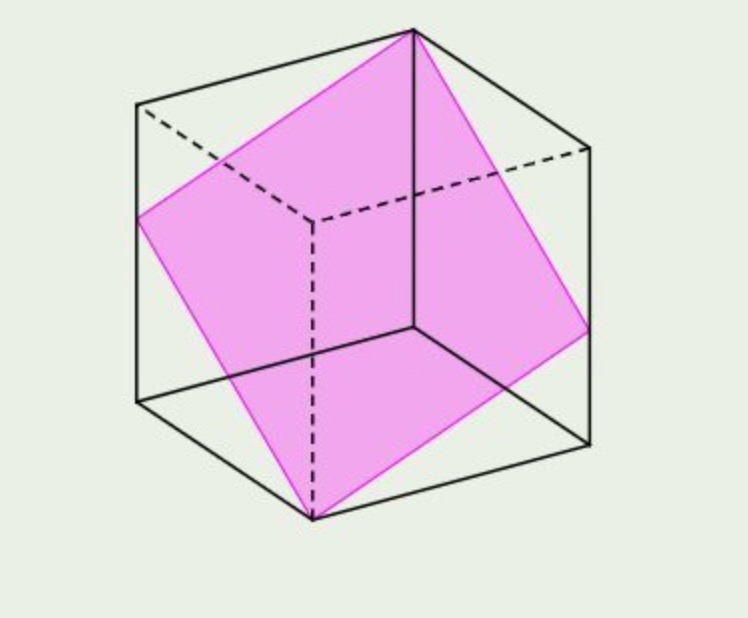
\includegraphics[scale=0.20]{graph.jpg}
%    \end{center}
% OR: 
%\begin{figure}
%    \centering
%    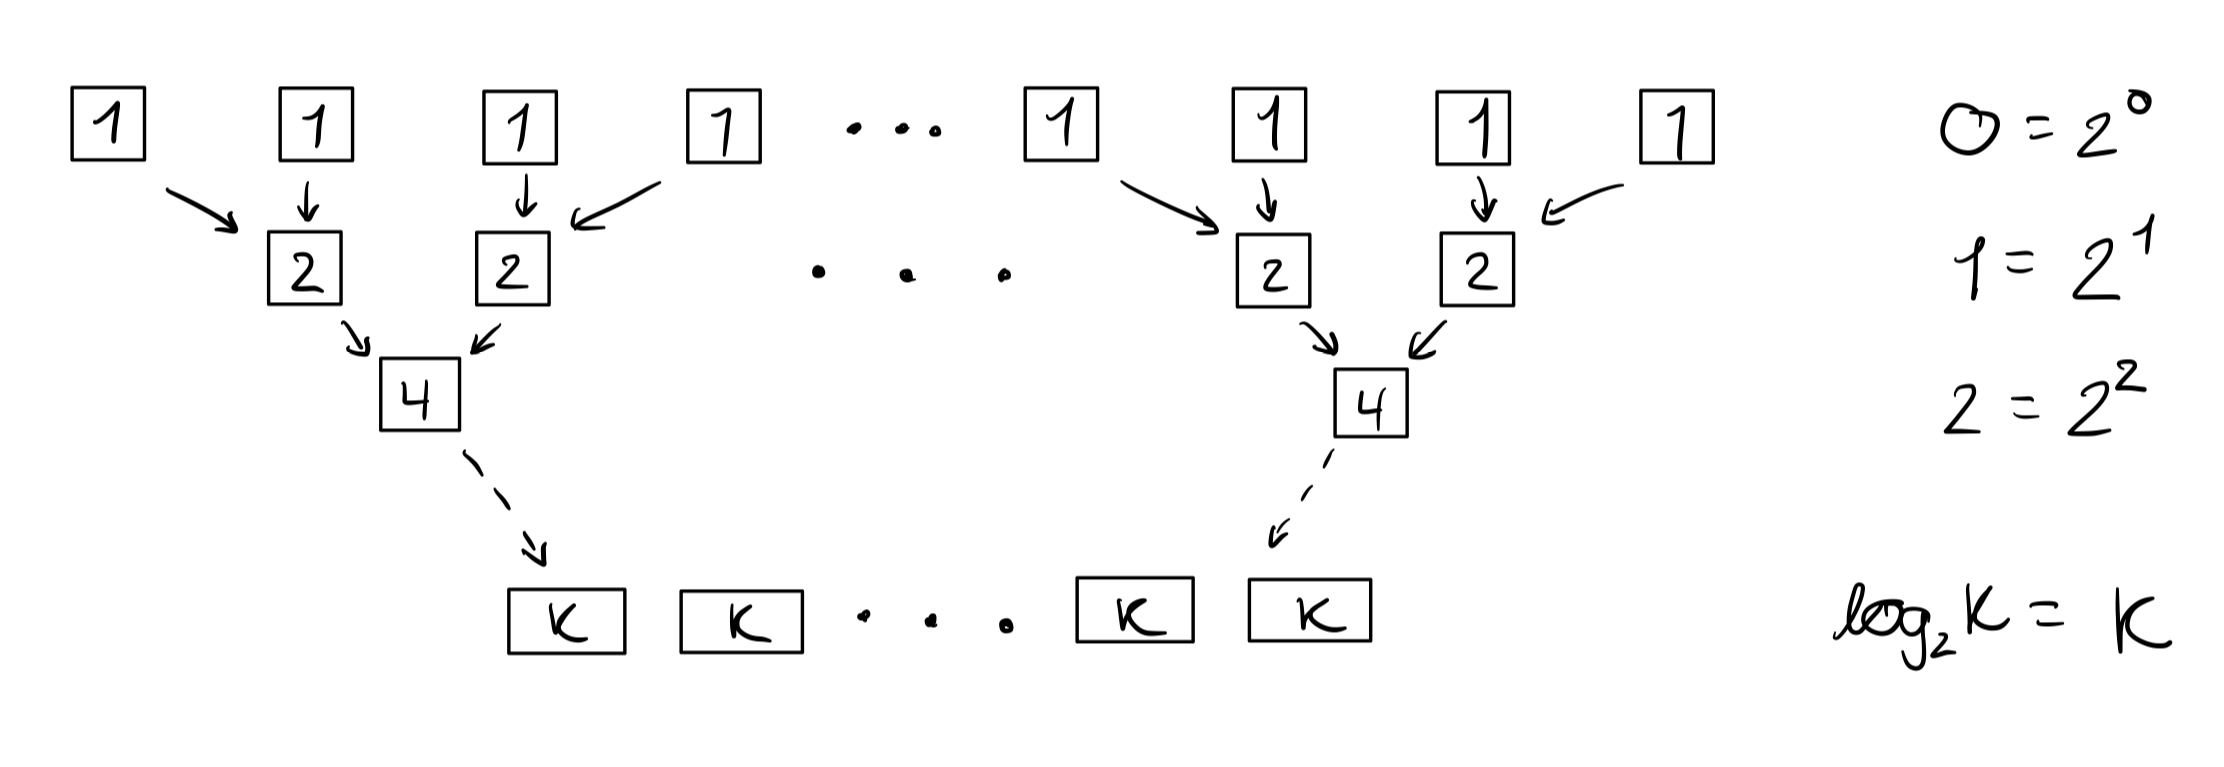
\includegraphics[scale=0.20]{IMG_1052.jpg}
%    \caption{Your caption text here.}
%\end{figure}


%macros for recursive functions
%For plots
\usepackage{pgfplots}
\pgfplotsset{compat = newest}

\newtheorem{theorem}{Theorem}
\declaretheoremstyle{lemma}
\declaretheorem[style=lemma, name=Lemma]{lemma}

\theoremstyle{definition}
\newtheorem{definition}{Definition}

\declaretheoremstyle{example}
\declaretheorem[style=example, name=Example]{example}

\theoremstyle{remark}
\newtheorem*{remark}{Remark}

\declaretheoremstyle{proposition}
\declaretheorem[style=proposition, name=Proposition]{proposition}

\declaretheorem[name=Note]{note}
\declaretheoremstyle{note}

\setlength\parindent{24pt}%set paragraph indent

\newenvironment{ftheo}
  {\begin{mdframed}\begin{theorem}}
  {\end{theorem}\end{mdframed}}


  % --- Special commands --- %
\newcommand\sol{%
  \\ 
  \\
  \textit{Solution:}\\%
}
% Statistics
\newcommand{\indep}{\perp \!\!\! \perp}
\DeclareMathOperator{\var}{Var}
\DeclareMathOperator{\cov}{Cov}

%Convex optimisation operators
\DeclareMathOperator{\cl}{cl}
\DeclareMathOperator{\epi}{epi}
\DeclareMathOperator{\lev}{lev}
\DeclareMathOperator{\dom}{dom}
\DeclareMathOperator{\aff}{aff}
\DeclareMathOperator{\ri}{ri}
\DeclareMathOperator{\argmin}{argmin}

% --- Algos --- %
\SetKwProg{Fn}{Function }{\string:}{}

% --- Header --- %
\renewcommand{\headrulewidth}{.4mm} % header line width

\pagestyle{fancy}
\fancyhf{}
\fancyhfoffset[L]{1cm} % left extra length
\fancyhfoffset[R]{1cm} % right extra length
\rhead{\today}
\lhead{\it Alexandre St-Aubin (261115785) \& Dylan Telio (261119191)}
\rfoot{}

% --- Title Page --- % 
\setlength{\droptitle}{-6em}

\title{\textsc{Assignment 3 -- COMP 252}}  
\author{\it Alexandre St-Aubin (261115785) and Dylan Telio (261119191)}
\date{\today}

\begin{document}
\maketitle 
\begin{enumerate}
  \item \textsc{Decision tree lower bound.}
  \begin{enumerate}
    \item[\it (i)]Give a simple algorithm for this problem and an upper bound on the complexity. For n = 5, your answer should be 7.
    \sol
    \begin{algorithm}
    \caption{An algorithm to classify the $n$ monkeys. }
    \SetKwRepeat{Do}{do}{while} %do-while loop macro
    \SetKwInput{KwOut}{Output}
    \SetKwInput{KwIn}{Input}
    \SetKwData{monk}{Monkeys}
      \SetKwData{app}{append}
    \SetKwData{typea}{Species\_1}
    \SetKwData{typeb}{Species\_2}
    \SetKwData{typec}{Species\_3}
    \KwIn{An array \monk of monkeys.}
    \KwOut{Three arrays separating the monkey species.}
    \BlankLine
    \typea $\leftarrow$ new Array;  \\ 
    \typeb $\leftarrow$ new Array;  \\ 
    \typec $\leftarrow$ new Array;  \\ 
    $i \leftarrow 1;$\\ 
    $\typea.\app(\monk[0])$;\\
      \While{$\monk[0] = \monk[i]$}{
        $\typea.\app(\monk[i])$; \\ 
        $i++;$\\ 
      }
      \tcp{loop above exits only if a second monkey species was found}
      $\typeb.\app (\monk[i]);$
    \BlankLine 
      \tcp{for each remaining monkey, compare to the 2 known species}
      \For{$j$ in range $[i, n]$ }{
      \If{$\monk[j] = \typea[0]$}{
      \typea.\app(\monk[j]);
      }\ElseIf{$\monk[j] = \typeb[0]$}{
      \typeb.\app(\monk[j]);
      }\Else{
      \typec.\app(\monk[j]);
      }
      }
  \end{algorithm}
    \begin{remark} 
      The worst case for the above algorithm is when the two first monkeys are different, and each remaining monkey is of the third or second species, hence must be compared twice (once to each of the first two species), in order to be classified. This yields an upper bound complexity of $1 + 2(n-2).$ When $n = 5, $ this is indeed equal to 7.
    \end{remark} 
    \newpage
    \item[\it (ii)] Show that all leaves in the decision tree must be different (i.e., correspond to different outputs).
\begin{proof} 
    Fix a sequence of monkeys. The decision tree representing the algorithm described in part $(i)$ is binary, where each decision takes as input two monkeys, and outputs whether they are of the same species or not. Every monkey must be compared at most twice to be classified. We can represent each comparison by a bit, 1 being a match, and 0 otherwise. The output for a given monkey will therefore be: 
   $$\left\{ \begin{matrix}
     10 & \text{ if match with Species\_1} \\ 
01 & \text{ if match with Species\_2} \\ 
00 & \text{ if match with Species\_3} 
   \end{matrix} \right.$$
    We note that in reality, if there is a match with Species\_1, the monkey will not be compared with the other species, as it would be useless. So, the notation $10$ is not entirely representative of what truly happens in the algorithm, it should rather be $1$, as only one comparison is made. However, for sake of notation, we keep it as $10.$

    \hspace{24pt}Hence, one easily sees that each leaf in the decision tree can be represented as a binary sequence of comparisons, where each 2 consecutive bits represents the classification of a monkey. In order to relax notation, let $10 = 1, \; 01 = 2,\; 00 = 3 $, then each leaf is given as a sequence of the form
    $$1233322123123121$$
    We show by induction that each leaf represents a unique monkey sequence. The base case is clear when $n =2$. Now, assume that for $n-1$ monkeys, each leaf is represented by a unique sequence of the numbers $\{1,2,3\}$ of length $n-1$. Then, if we add a monkey to the end of the array of monkeys, for each existing sequence $\{a_i\}_{i=1}^{n-1}$, 3 sequences of length $n$ will be created: 
    $$a_{i,1} := \{a_i\}_{i=1}^{n-1}\cup \{a_n = 1\}  $$
  $$a_{i,2} := \{a_i\}_{i=1}^{n-1}\cup \{a_n = 2\}  $$
  $$a_{i,3} := \{a_i\}_{i=1}^{n-1}\cup \{a_n = 3\}  $$

  Clearly the 3 new sequences are unique for each $i$, and since the $n-1$ first elements of every sequence are unique by the induction hypothesis, it follows that all of the sequences representing the decision tree for $n$ monkeys are unique. Hence, the leaves represent unique outputs. 

\end{proof}
     \item[\it (iii)] Using a decision tree-based method, show that the lower bound for this problem is 6 when $n = 5$.
     \begin{proof} 
      The algorithm outputs three sets of monkeys of identical species. For each monkey, there are three possibilities of species, hence $3^5$ total permutations. Yet, this accounts for the order of the species, which we don't care about. That is, it shouldn't matter whether the \textit{popa langurs} are grouped in Species\_1, Species\_2, or Species\_3. To remove this unwanted notion of order, we divide by $3!$. It follows that the total number of possible outputs for this problem is given by
    $$\frac{3^n}{3!} $$
       By part (ii), each leaf corresponds to a different output, so we have a tree with $\frac{3^n}{3!}$ leaves. Thus, by the method of decision trees, the lower bound is
    $$\left\lceil\log_{2}\left( \frac{3^5}{3!} \right)\right\rceil = 6$$
       In reality, we might be removing too many leaves by dividing by $3!$, as not every grouping of monkeys is seen $3!$ times, i.e. $(3,1,1)$ occurs only $3$ times, not $3! = 6.$ However, this doesn't matter, as by assuming less leaves, we achieve a lower lower bound.
     \end{proof}
  \item[\it (iv)] For general $n,$ show that the decision tree lower bound is at least $an- b$ and at most $an + b$
    for $n \geq n_0$, for some positive numbers $a, b, n_0$. Determine suitable values for these numbers. Compare this with your answer in \textit{(i)} and conclude that the decision tree bound for this problem is rather weak.
    \sol 
     For a general $n,$ the number of leaves in the decision tree is upper bounded by $3^n$, because there are 3 possible groups that each monkey can be placed in. However, two leaves may correspond to the same permutation of monkeys, which will result in less than $3^n$ leaves, but it remains an upper bound. A lower bound for the number of leaves is $\frac{3^n }{3!} $, which assumes that for each grouping of monkeys, all permutations of this outcome appear as a unique leaf in the decision tree. With at most $3^n$ leaves, the decision tree lower bound is at most $$\lceil \log_2 (3^n)\rceil = \lceil n \log_2 3\rceil \leq n \log_2 3 + \log_2 6 $$ 
     With at least $\frac{3^n}{3!} = \frac{3^n }{6} $ leaves, the decision tree lower bound is at least $$\left\lceil\log_2 \frac{3^n}{6} \right\rceil = \left\lceil n \log _2 3 - \log_2 6 \right\rceil \geq n \log _2 3 - \log _2 6, $$
     thus $a = \log_2 3 $ and $b = \log_2 6$, and for the decision tree lower bound (DCB), we have 
     $$an -b = n\log_2 3  - \log_2 6 \leq \text{DCB} \leq n \log_2 3 + \log_2 6 = an +b  $$
   
    This decision tree bound is rather week, as for $n =5$, it is at most $5 \log_2 3 + \log_2 6$, which is approximately $10.5$, i.e., way more than the algorithm found in part (i) which had a complexity of 7. 

     \end{enumerate}
  \newpage
  \item \textsc{Adversarial lower bound.} Using the method of adversaries, show that the lower bound for this problem is 7 when $n = 5$. 
  \sol 
  \textsc{Adversary Strategy:} The adversary always answers NO, unless it has to answer YES.

  \textbf{Claim}: This strategy always yields at least 7 comparisons.
  \begin{proof} 
    Denote the set of monkeys by $\Omega := \{a,b, c,d,e\}$. There are two cases where the adversary must answer "yes" to a comparison between two monkeys. Without loss of generality, let $a \in $ Species\_1 and $x\in \Omega$, then the adversary will be forced to answer yes if,
    \begin{enumerate}
      \item[\it (i)] $x$ was already compared to Species\_2 and Species\_3, and the adversary answered "no" to both.
      \item[\it (ii)] $x$ was already compared to Species\_1 and the adversary answered "yes". 
    \end{enumerate}
    Notice that in either case, the algorithm doesn't gain any new information. We may therefore assume that the adversary will never be forced to answer "yes", as any good algorithm would not waste comparisons to obtain information it already knows. 
    
    \hspace{24pt}Therefore, our claim is that no matter the comparisons asked (except those that are useless, as above), answering "no" to each will always require at least 7 comparisons before the 5 monkeys are classified. We prove this using \textit{brute force}, i.e. by trying to find a way for the 5 monkeys to be correctly classified in 6 comparisons, failing to do so, and concluding that at least 7 will be required. Since classifying the first 2 monkeys always takes just one comparison, the remaining 3 monkeys must therefore be classified with 5 comparisons. Let,
    \begin{enumerate}
      \item $X : =\{a, b\}$ be the two monkeys compared at first;  
      \item $Y:= \{c,d,e\}$ the 3 remaining monkeys that need to be classified. 
    \end{enumerate}

    We call \textit{internal} the comparisons that are made within $Y$, and \textit{external} those that are made between $X$ and $Y$. Making only external comparisons is equivalent to the algorithm in $(i)$, and clearly yields 6 additional comparisons (2 for each of $\{c,d,e\}$). So, we try and make internal comparisons. Without loss of generality\footnote{The reason why it's \textit{wlog} is that the order that the comparisons are made does not matter, and nor does which monkeys they are made between (by relabelling).}, there are 3 possible strategies: 
    \begin{enumerate}
      \item[\it (i)] 3 internal comparisons: $c\&d, \; d\&e, e\&c$ to obtain that they are all different species. But then at least 3 external comparisons will be required to classify them: $c\&a,\; c\&b,\; d\&a$ (recall that each comparison returns "not equal" by our chosen adversary). 
      \item[\it (ii)] 2 internal comparisons: $c\&d, \; d\&e$ to get that $c\neq d$, $d \neq e$ and $e?d.$ Then, 4 external comparisons must be made: $c\&a,\; c\&b, \;d\&a,\; e\&a.$
      \item[\it (iii)] 1 internal comparison: $c\&d$, similarly requires 5 external comparisons with $a, b.$
    \end{enumerate}
    Hence, the claim holds and by the adversary method, we conclude that the lower bound for the problem is 7 when $n=5.$
  \end{proof}


  \newpage
  \item \textsc{Lower bounds by the method of adversaries, and an algorithm.} Let the data
consist of an $n \times n\times n$ matrix of different integers that are sorted along all three axes from small to large. We have a ternary comparison oracle at our disposal. For a given integer $x$, we are asked to verify whether $x$ is an element of the matrix. The only comparisons that are allowed are between $x$ and matrix elements. 
\begin{enumerate}
  \item[\it (a)] Using the method of adversaries, derive a lower bound (called $L(n)$) for the worst-case number of times the oracle has to be consulted to perform a successful search for $x$. 
  \sol 
  We first define an adversary strategy for the $2D$ case. Suppose you have a $n\times n$ ordered matrix of the form: 
  $$A = \begin{pmatrix}
    a_{1,1} & a_{1,2} & a_{1,3} & \hdots & a_{1,n} \\ 

    a_{2,1} & a_{2,2} & a_{2,3} & \hdots & a_{2,n} \\ 

    a_{3,1} & a_{3,2} & a_{3,3} & \hdots & a_{3,n} \\ 
    \vdots & \vdots & \vdots & \ddots & \vdots \\ 
    
    a_{n,1} & a_{n,2} & a_{n,3} & \hdots & a_{n,n} \\ 
  \end{pmatrix}$$
  Where $a_{1,1}$ is the smallest entry and $a_{n,n}$ the greatest. 

  \textsc{2D Adversary strategy:} when asked to compare $x$ with the entry $a_{i,j}$, the adversary will answer : 
  \begin{enumerate}
    \item $(x > a_{i,j})$, if $i + j \leq n + 1$; 
    \item $(x < a_{i,j})$, if $i+ j > n+ 1$; 
    \item $(x = a_{i,j})$, if $a_{i,j}$ is the last element left in the matrix. 
  \end{enumerate}
  In other words, if the algorithm asks about a matrix entry below the \textit{bottom-left to top-right diagonal,} answer \textbf{smaller}, and if it is on, or above it, answer \textbf{greater}. 
    \begin{remark}[1]
    We say an entry $a_{i,j} \in A$ is \textit{removed} from $A$ when the adversary confirms that it is not equal to $x$.   
  \end{remark}
  \begin{remark}[2]
    Notice that if the algorithm asks about $a_{i,j}\in A,$ and that $i + j \leq n + 1$, then for every $k\leq i, \; l \leq j,$ $a_{k,l}$ will be removed. 
  \end{remark}
  \hspace{24pt}Now, by the way our adversary is defined, from the point of view of the algorithm, the only way to remove elements of the \textit{bottom-left to top-right diagonal} is to compare each of its entries to $x$. This process is also sufficient to remove the upper left half of the matrix. Thus, removing every entry $a_{i,j}$ such that $j+ i \leq n+1$ takes \textbf{at least} $n$ steps. By an analogous argument, removing the remaining entries will take at least $n-1$ steps (by comparing $x$ with each entry directly below the diagonal). 
  Therefore, this adversary gives a lower bound of $2n -1.$
  \begin{remark}[3]
    An alternate way to view the above adversary is that it picks the answer that minimizes the area of the square of entries removed.
\end{remark}
  \textsc{3D Adversary strategy:} We use a similar strategy as in the 2D case, but instead of minimizing an area, as stated in \textit{Remark 3}, we minimize a volume. Let $\Omega = \{<, >, =\}$, and let 
  $$F: [1,n]\times [1, n]\times [1,n] \subseteq \mathbb{N}^3 \to \Omega $$
be given by 
  $$F(i,j,k) = 
  \begin{cases}
    <, &\text{ if } i \times j \times k \leq (n+1 - i )\times (n+1 - j ) \times (n+1 -k) \\ 
    >, &\text{ if } i \times j \times k > (n+1 - i )\times (n+1 - j ) \times (n+1 -k) \\ 
    =, &\text{ if } a_{i,j,k} \text{ is the last entry not removed. }
  \end{cases} $$
  where $F$ is exactly our adversary for the 3D case. 

  \textbf{Claim :} The adversary defined by $F$ gives a lower bound of $O(n^2).$ 

  
  The set of points that must be checked looks similar to the purple plane in figure 1. The area of this plane is $O(n^2)$. The reason why all points on this plane must be checked is that they are the ones that won't be removed unless they are checked directly.
 \begin{figure}
\label{matrix}
    \centering
    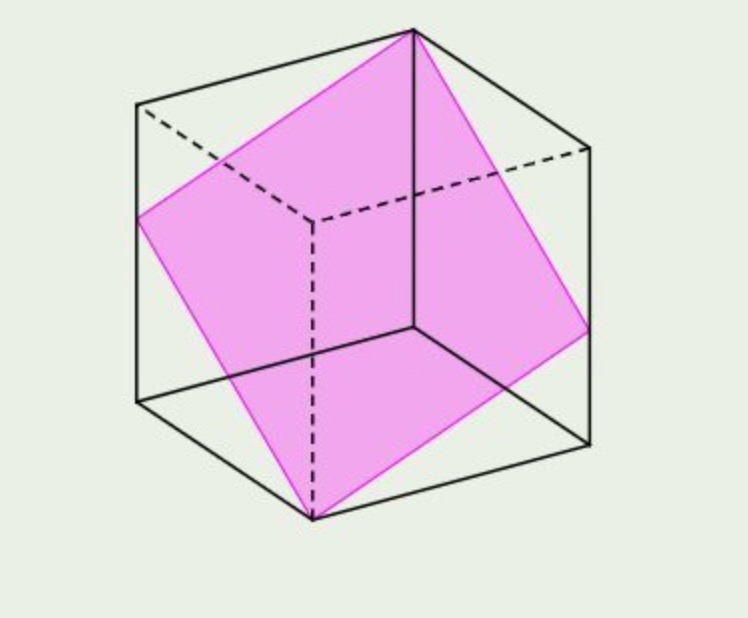
\includegraphics[scale=0.40]{graph.jpg}
    \caption{  }
\end{figure}
  \newpage 
  \item[\it (b)] Give an algorithm that takes worst case time $O(L(n))$. 
  \sol 
  \begin{algorithm}
    \caption{An algorithm to find if $x$ is in a 3D ordered matrix, in $O(L(n))$. }
    \SetKwRepeat{Do}{do}{while} %do-while loop macro
    \SetKwInput{KwOut}{Output}
    \SetKwInput{KwIn}{Input}
    \SetKwFunction{matsolve}{Is\_x\_in\_this\_2D\_Matrix}
    \SetKwData{mat}{Matrix\_2D}
    \SetKwData{x}{x}
    \SetKwData{col}{col}    
    \SetKwData{row}{row}   
    \SetKwData{true}{True}   
    \SetKwData{false}{False}   

    \KwIn{ A sorted $n \times n \times n$ matrix $M$ of unique integers and an integer $x$. That is, $M[0][0][0]$ is the smallest element and $M[n-1][n-1][n-1]$ the biggest. }
    \KwOut{True or False, whether $x \in M$}
    \BlankLine

    \Fn{\matsolve{\mat}}{
    \tcp{start the iteration at top right corner of matrix}
    $\row \gets 0$;\\ 
    $\col \gets n-1 $ ; \\  
    \While{$\col \geq 0 \text{ and } \row \leq n-1$}{
      \If{$\x = \mat[\row][\col]$}{
      \Return \true;
      }\ElseIf{$x< \mat[\row][\col]$}{
      $\col \gets \col -1$; 
      }\Else{
      $\row \gets \row + 1$; 
      }
      }\Return \false;
    }
    \BlankLine
    \tcp{ go through each 2D matrix in the 3D matrix, starting with the top one.}
    \For{all $k \in [0,n-1]$}{
    \tcp{if x > M[n-1][n-1][n-1], no need to check this 2D matrix}
    \If{$\x \leq M[n-1][n-1][n-1]$}{
      \If{\matsolve{M[k]}}{
      \Return \true;
      }
    }
    }\Return \false;
   
    
  \end{algorithm}
  \begin{remark} 
    In the above algorithm, the time complexity of the function at line 1 is easily seen to be $O(n)$, as it takes at most $2n$ steps. Now, since this function will be called at most $n$ times (once for each level of the 3D matrix), we conclude that the overall time complexity of the algorithm is $O(n^2)$, as desired. 
\end{remark}

\newpage 
\begin{figure}
\label{matrix}
    \centering
    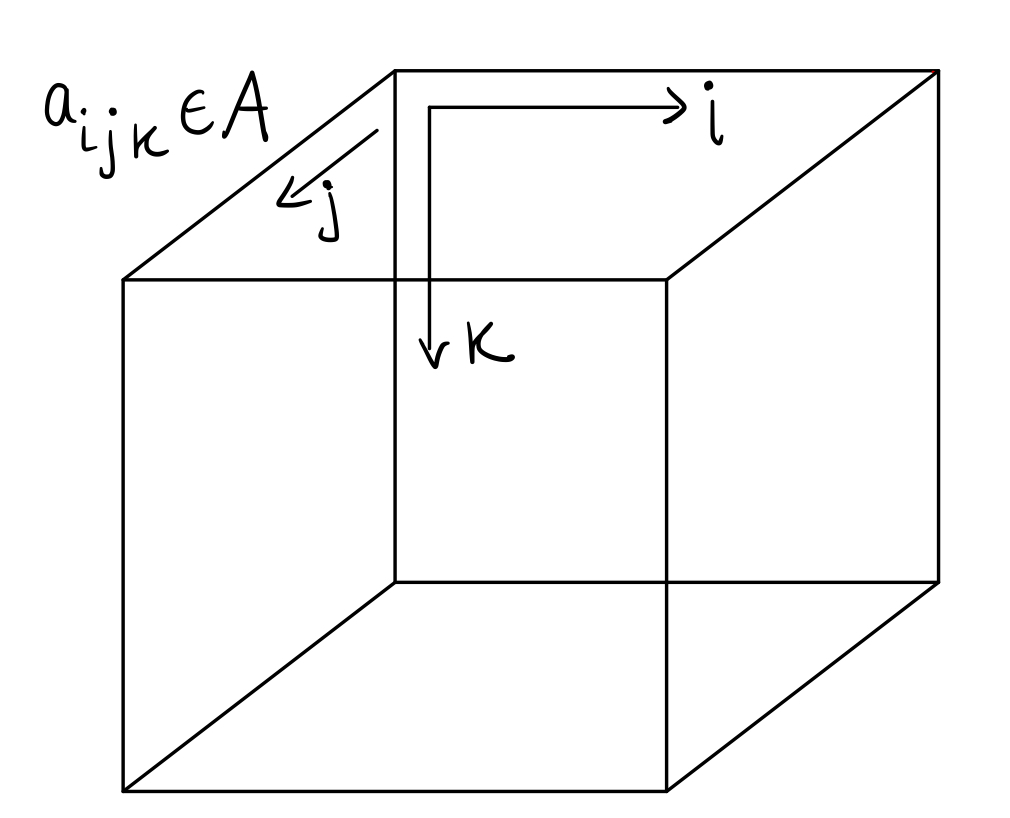
\includegraphics[scale=0.20]{3dmatrix.jpg}
    \caption{The 3D matrix in problem 3.}
\end{figure}

\end{enumerate}
\end{enumerate}
\end{document}
